\documentclass[11pt, a4paper, sans, colorlinks, linkcolor=True]{moderncv}
\moderncvstyle{classic}
\moderncvcolor{black}
\usepackage{ragged2e}
\usepackage[utf8]{inputenc}
\usepackage{enumitem}
\usepackage[left=1in, right=1in, bottom=0.5in, top=0.5in]{geometry}
%\addtolength{\topmargin}{-.875in}
\pagenumbering{gobble}
\usepackage{setspace}

%Personal Details
\name{Oliver James}{Hall}
\title{Coverletter}
\address{School of Physics and Astronomy\\ University of Birmingham, Edgbaston}{B15 2TT, Birmingham}{United Kingdom}
\email{ojhall94@gmail.com}
\homepage{https://www.ojhall94.github.io}


\begin{document}
\definecolor{links}{HTML}{3f28bd}
\hypersetup{urlcolor=links}
\recipient{\ }{\ }
\date{\today}
\opening{Dear Nature Astronomy editors,}
\makelettertitle
\justify
\vspace{-0.5cm}

We have written a paper where we use asteroseismology -- the study of oscillating stars -- to gain a new understanding of stellar rotational evolution in stars like the Sun. Using a novel ensemble of asteroseismic rotation, we provide very strong evidence of the existence of the much-debated theory of weakened magnetic braking. This represents a major leap forward for the field of stellar rotational evolution, using rotation measurements independent of those used to first propose the theory, and including older, inactive stars. We think it would be a good fit for your journal, and hope you agree. We have provided a concise summary below.\\

As cool main sequence stars like the Sun grow older, their rotation slows down as magnetic winds carry away angular momentum. The study of this age-rotation relationship, called gyrochronology, provides much potential for measuring stellar age from a star’s rotation, down to 10\% [1]. However gyrochronology has major problems for older stars. A 2016 study, published in Nature, used ages determined through asteroseismology to show that stars older than the Sun appeared to stop losing angular momentum [2]. This effect, which deeply complicates the use of gyrochronology for older stars, was dubbed “weakened magnetic braking”.

{\hskip 1em}Since it was initially proposed, the idea of weakened magnetic breaking has received widespread attention from the stellar astrophysics community. Whether this phenomenon  actually takes place on the main sequence is currently uncertain. Stellar rotation is typically measured by looking at star spots on the surface. Since older, inactive stars show fewer spots, a lack of slow rotation rates on the main sequence may in fact be a selection effect, and not a physical reduction in angular momentum loss [3]. 

{\hskip 1em}Our study solves this lack of rotation rates for inactive stars by measuring rotation using asteroseismology. Modes of oscillation will rotationally shift in frequency due to a star’s spin, allowing us to measure rotation independent of activity. Asteroseismic rotation has been shown to be a good proxy for surface rotation (something we re-confirm in our paper). In fact you might even consider it to be more fundamental than spot rotation.

{\hskip 1em}In our study, we measured inclination angles and seismic rotation of 91 main sequence stars. These measurements form the largest legacy catalogue of seismic rotation to date, as well as the largest sample of surface rotation of inactive main sequence stars until the launch of PLATO. We compared these new rotation rates to models of stellar rotational evolution, and found that our ensemble overwhelmingly favoured a model where weakened magnetic braking took place. By demonstrating that weakened magnetic braking is needed using seismic rotation for a sample that includes inactive stars, we open the doors for a new era of understanding of the interactions between age, magnetism and rotation in the Sun and stars like it.\\

We believe this work will interest your diverse readership, for a number of reasons:
\begin{itemize}[leftmargin=1.5em]
\itemsep0em 
\item[--] It uses new data -- the first large ensemble of asteroseismic rotation -- to settle an ongoing problem in gyrochronology and stellar modelling, and represents a major result in the field of stellar rotation.

\item[--] It presents novel techniques, determining stellar rotation from interior sound waves that form modes of oscillation on the surface, and assessing two stellar models simultaneously in a Bayesian mixture model framework.

\item[--] Our rotation catalogue and confirmation of weakened magnetic braking together form an important stepping stone in how late main sequence ages may be determined in the near future. This will be interesting to a wide range of astronomers that are looking to find well-constrained ages of stars (e.g. to study planets, stars, clusters and the Milky Way, as well as to constrain stellar evolutionary theory).

\item[--] The Sun is currently thought to lie close to the boundary where weakened magnetic braking kicks in [2]. Our findings affect the predicted rotational evolution of the Sun, and with it, the Sun’s future levels of activity.
\end{itemize}

The cross-disciplinary nature of our study (asteroseismology and rotational evolution) means we have a wide range of expert referees we can suggest.

\begin{itemize}[leftmargin=1.5em]
\itemsep0em 
\item[--] \href{https://fys.kuleuven.be/ster/staff/conny-aerts}{Conny Aerts} - asteroseismology and statistics. 
\item[--] \href{https://ruthangus.github.io/}{Ruth Angus} - applied gyrochronology and Bayesian statistics
\item[--] \href{https://www2.physics.ox.ac.uk/contacts/people/aigrain}{Suzanne Aigrain} - Bayesian statistics, stellar rotation and gyrochronology. Good knowledge of asteroseismology.
\item[--] \href{https://www.aip.de/Members/sbarnes/dr.-sydney-barnes}{Sydney Barnes}* - stellar rotation and gyrochronology calibration
\item[--] \href{https://www.fgcu.edu/directory/dbuzasi?list=1}{Derek Buzasi}** - theoretical and observational gyrochronology, asteroseismology
\item[--] \href{https://www.unige.ch/sciences/astro/evolution/en/members/patrick-eggenberger/}{Patrick Eggenberger} - asteroseismology, angular momentum transport in stellar interiors
\item[--] \href{https://www.mpg.de/5040011/sonnensystemforschung_wissM7}{Laurent Gizon} - stellar rotation, asteroseismology and asteroseismic modelling
\item[--] \href{https://www.iau.org/administration/membership/individual/6822/}{Marie-Jo Goupil} - stellar evolutionary theory
\item[--] \href{https://www.physastro.iastate.edu/directory/sdk}{Steve Kawaler} - stellar rotational evolution and asteroseismology
\item[--] \href{https://orcid.org/0000-0001-5928-7251}{Nuccio Lanza} - stellar rotation
\item[--] \href{https://astronomy.fas.harvard.edu/people/soren-meiborn}{Soren Meibom} - gyrochronology and surface rotation
\item[--] \href{https://whitedwarf.org/travis/}{Travis Metcalfe}*** - asteroseismology, stellar rotation and stellar activity
\item[--] \href{https://www.stsci.edu/stsci-research/research-directory/david-soderblom}{David Soderblom} - stellar ages and activity
\end{itemize}

* Known to be skeptical of weakened magnetic braking which is in opposition to his own research. Previous encounters as a referee with the authors have been difficult and less than constructive.

** Has provided references for me in the past.

*** Frequently collaborates with the third author on studies of stellar rotational evolution.\\

We hope you enjoy our paper, and that you consider publishing it in your journal. We think it would be an excellent fit, as it uses a new and unique cross-disciplinary analysis to end a long-standing discussion in the field of stellar rotational evolution.

\vspace{0.5cm}

Yours sincerely, \\
\vspace{0.5em}
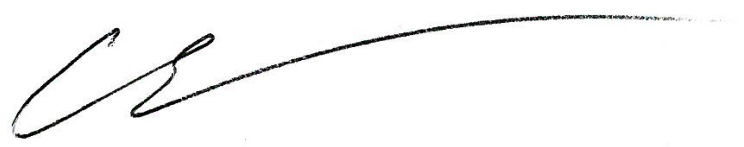
\includegraphics[scale=0.2]{signature.png} \\ 
\vspace{0.5em}
\textbf{Oliver J. Hall}, on behalf of the authors. \\

References:

{\hskip 1.5em}[1] Meibom et al. (2015), \href{https://www.nature.com/articles/nature14118}{Nature}, 517, 589

{\hskip 1.5em}[2] van Saders et al. (2016), \href{https://www.nature.com/articles/nature16168}{Nature}, 529, 181

{\hskip 1.5em}[3] van Saders et al. (2019), \href{https://iopscience.iop.org/article/10.3847/1538-4357/aafafe}{The Astrophysical Journal}, 872, 128
\end{document}

